\documentclass[11pt,hyperref={bookmarks=false}]{beamer}
\usetheme{Warsaw}
%\usetheme{Madrid}
%\usecolortheme{beaver}
\usefonttheme{professionalfonts}
 \usepackage[usenames,dvipsnames]{pstricks}
 \usepackage{wallpaper}
 \usepackage{epsfig}
\definecolor{UniBlue}{RGB}{157,34,53}
\setbeamercolor{block title}{bg=UniBlue!70,fg=black}

\usepackage{psfrag,graphicx}
\usepackage{amsmath,amsfonts}
\usepackage{lscape}
\usepackage{array,epsfig}
\usepackage{amsfonts}
\usepackage{amssymb}
\usepackage{amsxtra}
\usepackage{amsthm}
\usepackage{makecell}
\usepackage[skip=0pt, belowskip=-10pt]{caption}
\usepackage{subcaption}
\usepackage{float}
\usepackage{multirow}
\usepackage{booktabs}
%\usepackage{subfigure}
\usepackage{eso-pic}
\usepackage{transparent}
\usepackage{graphicx}
\usepackage{tikz}
\usepackage{longtable}
\newtheorem{df}{Definition}
\newtheorem{lm}{Lemma}
\newtheorem{prp}{Proposition}
\newtheorem{sprf}{Sketch of Proof}
\newtheorem{prf}{Proof}
\newtheorem{conjecture}{Conjecture}
\newtheorem{suffc}{Sufficient Condition}
\setbeameroption{hide notes}
\newcommand{\threelinebracer}{$\left. \begin{array}{c} \\ \\ \\ \end{array} \right\rbrace$}
\newcommand{\threelinebracel}{$\left. \begin{array}{c} \\ \\ \\ \end{array} \right\lbrace$}
\newcommand{\twolinebracer}{$\left. \begin{array}{c} \\ \\ \end{array} \right\rbrace$}
\newcommand{\twolinebracel}{$\left. \begin{array}{c} \\ \\ \end{array} \right\lbrace$}
\newcommand{\bd}{\partial}

\usepackage{pgf}  
%\logo{\pgfputat{\pgfxy(-1.2,-0.2)}{\pgfbox[center,base]{\includegraphics[height=12pt, keepaspectratio]{UA_Logo_Horizontal.eps}}} }

%\usebackgroundtemplate
%{
  %  \node[opacity=0.3, at=(current page.south east),anchor=south east,inner sep=0pt] 
    %\includegraphics[width=\paperwidth,height=20pt]{UA_Logo_Horizontal.eps}%
%}

\linespread{1}
\usepackage{parskip}
%\setlength{\itemsep}{1em} 
%\addtolength{\parskip}{5pt}
\DeclareMathSizes{12}{10}{8}{6}
%  \begin{itemize}}{\end{itemize}}
% Separate slides by \begin{frame} and \end{frame}.
\title[Willingness-to-pay for Warnings]{Willingness-to-pay for Warnings: Some Tables}
\author[A. Gaduh, P. McGee and A. Ugarov]{A. Gaduh, P. McGee and A. Ugarov}
\institute[]{}
\date{\today}

\newcommand\BackgroundPic{%
\put(0,0){%
\parbox[b][\paperheight]{\paperwidth}{%
\vfill
\centering
%\includegraphics[width=\paperwidth,height=\paperheight,%keepaspectratio]{sancho.png}%
\vfill
}}}


\begin{document}
%\AddToShipoutPicture*{\BackgroundPic}

\begin{frame}
\titlepage
\end{frame}

%%%%%%%%%%%%%%%%%%%%%%%%%%%%%%%%%%%%%%%%%%%%%%%%%%%%%%%%%%%%%%%%%%%%%%%%%%%%%%%%%%%%%%%%%%%%%%%%
%%%%%%%%%%%%%%%%%%%%%%%%%%%%%%%%%%%%%%%%%%%%%%%%%%%%%%%%%%%%%%%%%%%%%%%%%%%%%%%%%%%%%%%%%%%%%%%%

\begin{frame}
\frametitle{Research Question}
\begin{itemize}
	\item How much do people value alerts (signals) about potential preventable threats?
	\item How do signal's probabilistic characteristics affect the willingness-to-pay for it and the welfare gains from using it?
	\item Applications:
	\begin{itemize}
		\item Natural disaster warnings (tornados, floods, earthquakes)
		\item Medical tests for treatable conditions
		\item Investing in research on likelihood of catastrophic events (rogue AI, global warming, pandemics)
	\end{itemize}
	\item Note: most real-life applications provide little practice with using the signal
\end{itemize}
\end{frame}


\begin{frame}
\frametitle{Overview of the Experiment}
\begin{itemize}
	\item An insurance experiment:
		\begin{itemize}
			\item Two states of the world: bad ($\omega=1$) and good ($\omega=0$)
			\item Probability of a bad state is $P (\omega=1) = \pi$
			\item Bad state $\implies$ loss of \$$L$
			\item A perfectly protective insurance can be purchased for \$$c$
		\end{itemize}
	\item Subject can purchase a signal $s$ before purchasing the insurance:
		\begin{itemize}
			\item A signal is characterized by its true-positive ($P(s=1|\omega=1)$) and true-negative rates ($P(s=0|\omega=0)$) 
		\end{itemize}
\end{itemize}

\vspace{1em}
\begin{block}{Research objective}
	How do signal characteristics affect the WTP?
\end{block}
\end{frame}


\begin{frame}
\frametitle{WTP for Signals}
\framesubtitle{If losses are rare ($\pi L<<c$)}

\begin{itemize}
	\item Theoretically, what should be the WTP for a signal?
	\item If bad states are a priori rare ($\pi L<<c$) $\implies$ never protect without a signal
	\item The theoretical WTP $b$ for an expected utility maximizer given a signal $s$ is a solution $b^*$ to the following:
	\small
		$$P(s=1)u(Y_0-b^*-c) + \pi P(s=0|\omega=1)u(Y_0-b^*-L)+$$
		$$+(1-\pi)P(s=0|\omega=0)u(Y_0-b^*) =(1-\pi)u(Y_0)+\pi u(Y_0-L)$$
\normalsize
	\item A risk-neutral agent then pays:
		\[b^*=\pi(1-P(s=0|\omega=1))L-P(s=1)c\]
\small
\end{itemize}
\end{frame}


\begin{frame}
\frametitle{WTP for Signals}
\framesubtitle{If losses are not necessarily rare}

\begin{itemize}
	\item The formulas become more complicated if subjects can protect without a signal (bad state are not rare enough)
	\item The theoretical WTP $b$ for an expected utility maximizer given a signal $s$ is a solution $b^*$ to the following:
	\small
 $$P(s=1)u(Y_0-b^*-c) + \pi P(0|1)u(Y_0-b^*-L)+(1-\pi)P(0|0)u(Y_0-b^*)=$$
		$$=\min[(1-\pi)u(Y_0)+\pi u(Y_0-L),u(Y_0-c)]$$

	\normalsize
	\item A risk-neutral agent then pays:
\small
		\[b^*=\min[\pi L,c]-\pi(1-P(s=0|\omega=1))L-P(s=1)c\]
\end{itemize}
\end{frame}



\begin{frame}
\frametitle{Hypotheses}
\begin{enumerate}
\item Conditional on the signal's value for risk-neutral subjects, false positive and false negative rates reduce the perceived value of the signal (WTP)
\item Conditional on the signal's value for risk-neutral subjects, false positive and false negative rates increase expected costs
\item Extra: how much of these disrepancies result from belief updating issues or risk aversion? 
\end{enumerate}
\end{frame}


\begin{frame}
\frametitle{WTP for signals}
\begin{itemize}
\item Higher average WTP for more valuable signals
\end{itemize}
\begin{figure}[h]
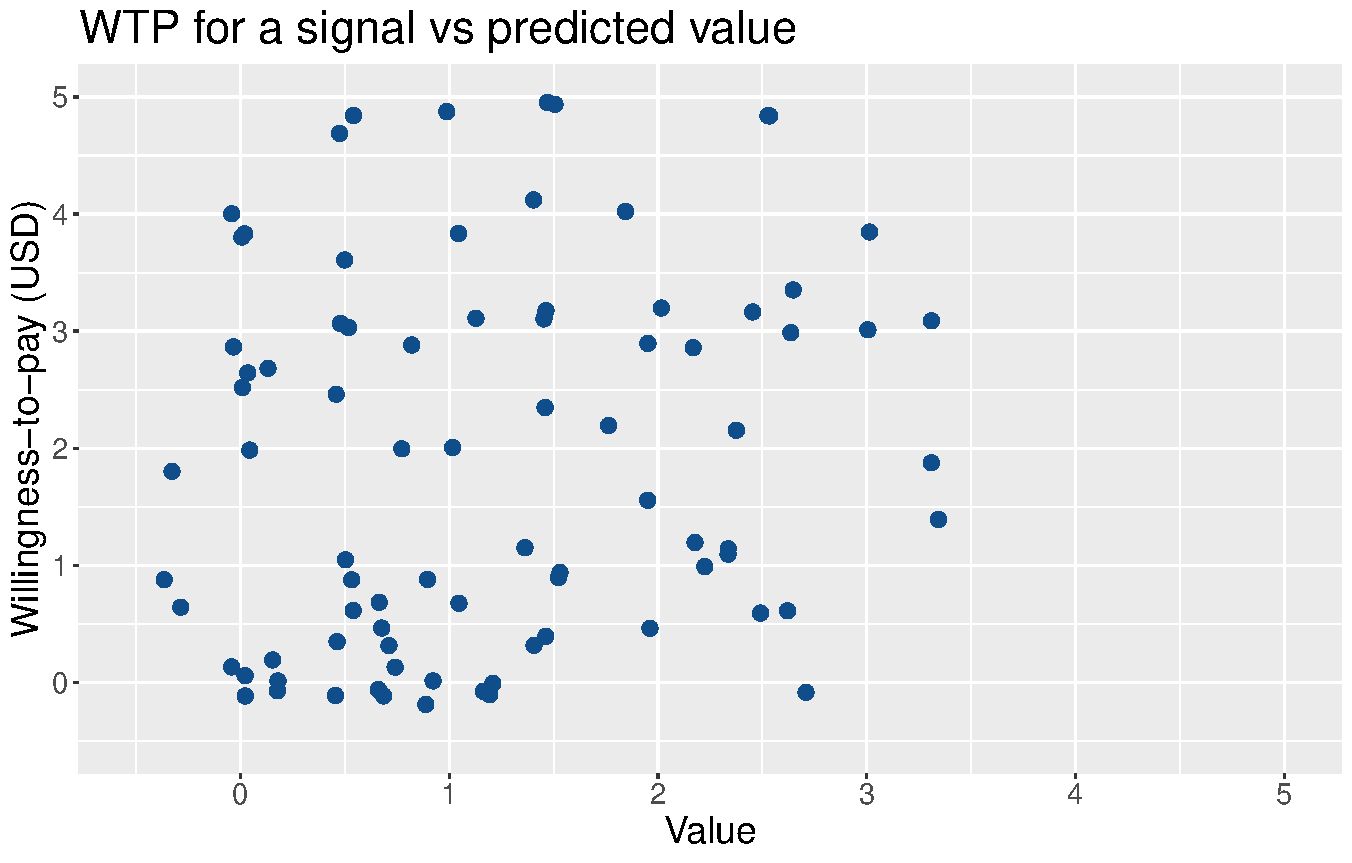
\includegraphics[scale=0.45]{Graphs/WTP_curve2.pdf}
\end{figure}
\end{frame}


\begin{frame}
\frametitle{WTP for the Signal}
\begin{itemize}
\item Extra effect of false positive and false negative rates
\end{itemize}

\footnotesize
\begin{table}[htbp]\centering
\def\sym#1{\ifmmode^{#1}\else\(^{#1}\)\fi}
\caption{WTP for Information}
\begin{tabular}{l*{5}{c}}
\hline\hline
                &\multicolumn{1}{c}{(1)}&\multicolumn{1}{c}{(2)}&\multicolumn{1}{c}{(3)}&\multicolumn{1}{c}{(4)}&\multicolumn{1}{c}{(5)}\\
                &\multicolumn{1}{c}{OLS}&\multicolumn{1}{c}{OLS}&\multicolumn{1}{c}{FE}&\multicolumn{1}{c}{FE}&\multicolumn{1}{c}{FE}\\
\hline
value           &     .688\sym{***}&      .71\sym{***}&     .713\sym{***}&     .381\sym{***}&     .135         \\
                &    (5.1)         &    (5.5)         &    (5.4)         &    (3.4)         &    (1.3)         \\
(sum) bp        &                  &    -.452\sym{***}&                  &                  &                  \\
                &                  &   (-4.3)         &                  &                  &                  \\
honest\_treatment&                  &                  &                  &     1.26\sym{***}&    -.248         \\
                &                  &                  &                  &    (3.1)         &   (-0.4)         \\
False neg. rate &                  &                  &                  &                  &    -3.94\sym{***}\\
                &                  &                  &                  &                  &   (-3.5)         \\
False pos. rate &                  &                  &                  &                  &    -6.08\sym{***}\\
                &                  &                  &                  &                  &   (-3.3)         \\
Constant        &     .961\sym{***}&     2.11\sym{***}&     .918\sym{***}&     1.07\sym{***}&     3.21\sym{***}\\
                &    (4.0)         &    (5.5)         &    (4.1)         &    (5.6)         &    (6.6)         \\
\hline
Observations    &      114         &      114         &      114         &      114         &      114         \\
Adjusted \(R^{2}\)&     0.18         &     0.25         &     0.29         &     0.41         &     0.53         \\
\hline\hline
\multicolumn{6}{l}{\footnotesize \textit{t} statistics in parentheses}\\
\multicolumn{6}{l}{\footnotesize \sym{*} \(p<0.10\), \sym{**} \(p<0.05\), \sym{***} \(p<0.01\)}\\
\end{tabular}
\end{table}

\end{frame}


\begin{frame}
\frametitle{WTP for the Signal (Risk Aversion)}
\begin{itemize}
\item Does accounting for risk aversion based on blind protection choices helps to explain WTP?
\end{itemize}
\footnotesize
\begin{table}[htbp]\centering
\def\sym#1{\ifmmode^{#1}\else\(^{#1}\)\fi}
\caption{WTP for Information (Accounting for Risk Aversion)}
\begin{tabular}{l*{5}{c}}
\hline\hline
                &\multicolumn{1}{c}{(1)}&\multicolumn{1}{c}{(2)}&\multicolumn{1}{c}{(3)}&\multicolumn{1}{c}{(4)}&\multicolumn{1}{c}{(5)}\\
                &\multicolumn{1}{c}{OLS}&\multicolumn{1}{c}{OLS}&\multicolumn{1}{c}{OLS}&\multicolumn{1}{c}{OLS}&\multicolumn{1}{c}{OLS}\\
\hline
value           &     .469\sym{***}&                  &                  &                  &                  \\
                &    (4.7)         &                  &                  &                  &                  \\
value\_ra        &                  &      .38\sym{***}&     .423\sym{***}&    .0872         &     .169         \\
                &                  &    (4.2)         &    (5.0)         &    (0.7)         &    (1.4)         \\
Prior prob.     &                  &                  &     2.95\sym{***}&                  &     2.72\sym{***}\\
                &                  &                  &    (4.2)         &                  &    (3.9)         \\
False neg. rate &                  &                  &                  &    -2.52\sym{***}&    -2.15\sym{***}\\
                &                  &                  &                  &   (-3.1)         &   (-2.7)         \\
False pos. rate &                  &                  &                  &    -2.05\sym{***}&    -1.79\sym{**} \\
                &                  &                  &                  &   (-2.6)         &   (-2.3)         \\
Constant        &     .977\sym{***}&     1.08\sym{***}&     .186         &     2.17\sym{***}&     1.19\sym{***}\\
                &    (5.5)         &    (6.1)         &    (0.8)         &    (5.5)         &    (2.7)         \\
\hline
Observations    &      228         &      228         &      228         &      228         &      228         \\
Adjusted \(R^{2}\)&     0.09         &     0.07         &     0.14         &     0.11         &     0.17         \\
\hline\hline
\multicolumn{6}{l}{\footnotesize \textit{t} statistics in parentheses}\\
\multicolumn{6}{l}{\footnotesize \sym{*} \(p<0.10\), \sym{**} \(p<0.05\), \sym{***} \(p<0.01\)}\\
\end{tabular}
\end{table}

\end{frame}


\begin{frame}
\frametitle{WTP for the Signal (Uniform Risk Aversion)}
\begin{itemize}
\item Risk aversion measurements are noisy. What if we assume the same risk aversion for everybody?
\end{itemize}
\begin{table}[htbp]\centering

\begin{tabular}{l c}
\hline\hline
                $\theta$ & $R^2$\\
\hline
0 &    .17       \\

0.5    &     .15\\

1 &     .1\\

1.5      &     .07   \\

\hline
Observations    &     150 \\
\hline\hline
\end{tabular}
\end{table}

\end{frame}


\begin{frame}
\frametitle{Actual Costs vs Theoretical Costs}
\begin{itemize}
\item Calculate actual costs based on decisions made in the Informed Protection treatment and actual posterior probabilities of losses.
\item Each reported participant's strategy $s$ is a tuple of numbers $(r_w,r_b)$ representing protection responses correspondingly to white and black hints
\item Then the expected cost of each decision are:
\small
$$EC(s)=\pi (P(0|1)(1-r_w)+P(1|1)(1-r_b))L+$$
$$+(P(s=0)r_w+P(s=1)r_b)c$$
\normalsize
\item Regress expected costs on minimal theoretical costs and other signal characteristics
\end{itemize}
\end{frame}


\begin{frame}
\frametitle{Actual Costs vs Theoretical Costs}
\footnotesize
\begin{table}[htbp]\centering
\def\sym#1{\ifmmode^{#1}\else\(^{#1}\)\fi}
\caption{Actual Exp. Costs vs Theoretical Costs}
\begin{tabular}{l*{6}{c}}
\hline\hline
                &\multicolumn{1}{c}{(1)}&\multicolumn{1}{c}{(2)}&\multicolumn{1}{c}{(3)}&\multicolumn{1}{c}{(4)}&\multicolumn{1}{c}{(5)}&\multicolumn{1}{c}{(6)}\\
                &\multicolumn{1}{c}{OLS}&\multicolumn{1}{c}{OLS}&\multicolumn{1}{c}{OLS}&\multicolumn{1}{c}{FE}&\multicolumn{1}{c}{FE}&\multicolumn{1}{c}{FE}\\
\hline
Optimal exp. costs&     1.04\sym{***}&     .842\sym{***}&     .592         &     1.04\sym{***}&     .879\sym{***}&     1.13\sym{***}\\
                &    (9.4)         &    (4.3)         &    (1.3)         &   (10.7)         &    (4.1)         &    (9.3)         \\
Prior prob.     &                  &    -2.19         &    -3.69         &                  &    -2.07         &                  \\
                &                  &   (-1.1)         &   (-1.2)         &                  &   (-1.1)         &                  \\
False neg. rate &                  &                  &    -2.68         &                  &                  &    -.696         \\
                &                  &                  &   (-1.6)         &                  &                  &   (-0.6)         \\
False pos. rate &                  &                  &     .713         &                  &                  &     2.51         \\
                &                  &                  &    (0.4)         &                  &                  &    (1.4)         \\
Constant        &    -.888\sym{***}&    -.733\sym{**} &    -.662\sym{**} &    -.875\sym{***}&    -.684\sym{***}&    -.918\sym{***}\\
                &   (-3.3)         &   (-2.6)         &   (-2.2)         &   (-4.0)         &   (-3.3)         &   (-4.3)         \\
\hline
Observations    &      150         &      150         &      150         &      150         &      150         &      150         \\
Adjusted \(R^{2}\)&     0.34         &     0.35         &     0.36         &     0.41         &     0.42         &     0.43         \\
\hline\hline
\multicolumn{7}{l}{\footnotesize \textit{t} statistics in parentheses}\\
\multicolumn{7}{l}{\footnotesize \sym{*} \(p<0.10\), \sym{**} \(p<0.05\), \sym{***} \(p<0.01\)}\\
\end{tabular}
\end{table}

\end{frame}


\begin{frame}
\frametitle{Additional Complementary Tables}
\begin{itemize}
\item Factors affecting informed protection responses
\item How well do participants update their beliefs?
\end{itemize}
\end{frame}



\begin{frame}
\frametitle{Informed Protection: Correlation}
\footnotesize
\begin{table}[htbp]\centering
\def\sym#1{\ifmmode^{#1}\else\(^{#1}\)\fi}
\caption{Informed Protection}
\begin{tabular}{l*{4}{c}}
\hline\hline
                &\multicolumn{1}{c}{(1)}&\multicolumn{1}{c}{(2)}&\multicolumn{1}{c}{(3)}&\multicolumn{1}{c}{(4)}\\
                &\multicolumn{1}{c}{All}&\multicolumn{1}{c}{All}&\multicolumn{1}{c}{Smart}&\multicolumn{1}{c}{Smart}\\
\hline
Posterior prob. &     .663\sym{***}&     .114         &     .692\sym{***}&     .126         \\
                &    (8.5)         &    (0.9)         &    (9.4)         &    (0.8)         \\
Prior prob.     &                  &     .467\sym{***}&                  &     .519\sym{***}\\
                &                  &    (3.5)         &                  &    (3.1)         \\
Gremlin says Black&                  &     .497\sym{***}&                  &     .506\sym{***}\\
                &                  &    (5.8)         &                  &    (5.0)         \\
Constant        &     .235\sym{***}&    .0872\sym{**} &     .233\sym{***}&    .0678         \\
                &    (7.3)         &    (2.2)         &    (7.7)         &    (1.6)         \\
\hline
Observations    &      300         &      300         &      228         &      228         \\
Adjusted \(R^{2}\)&     0.35         &     0.41         &     0.36         &     0.42         \\
\hline\hline
\multicolumn{5}{l}{\footnotesize \textit{t} statistics in parentheses}\\
\multicolumn{5}{l}{\footnotesize \sym{*} \(p<0.10\), \sym{**} \(p<0.05\), \sym{***} \(p<0.01\)}\\
\end{tabular}
\end{table}


\end{frame}



\begin{frame}
\frametitle{Informed Protection: Determinants}
\footnotesize
\begin{table}[htbp]\centering
\def\sym#1{\ifmmode^{#1}\else\(^{#1}\)\fi}
\caption{Informed Protection: Response to Reported Beliefs}
\begin{tabular}{l*{3}{c}}
\hline\hline
                &\multicolumn{1}{c}{(1)}&\multicolumn{1}{c}{(2)}&\multicolumn{1}{c}{(3)}\\
                &\multicolumn{1}{c}{All}&\multicolumn{1}{c}{All}&\multicolumn{1}{c}{Smart}\\
\hline
Belief          &     .746\sym{***}&     .358\sym{**} &     .462\sym{**} \\
                &    (7.8)         &    (2.4)         &    (2.5)         \\
Posterior prob. &                  &     .424\sym{***}&     .367\sym{**} \\
                &                  &    (3.5)         &    (2.6)         \\
Constant        &     .206\sym{***}&     .189\sym{***}&     .178\sym{***}\\
                &    (5.3)         &    (4.8)         &    (4.6)         \\
\hline
Observations    &      300         &      300         &      228         \\
Adjusted \(R^{2}\)&     0.32         &     0.38         &     0.40         \\
\hline\hline
\multicolumn{4}{l}{\footnotesize \textit{t} statistics in parentheses}\\
\multicolumn{4}{l}{\footnotesize \sym{*} \(p<0.10\), \sym{**} \(p<0.05\), \sym{***} \(p<0.01\)}\\
\end{tabular}
\end{table}

\end{frame}


\begin{frame}
\frametitle{Informed Protection: Do Subject's Beliefs Matter?}
\footnotesize
\begin{table}[htbp]\centering
\def\sym#1{\ifmmode^{#1}\else\(^{#1}\)\fi}
\caption{Informed Protection: Response to Reported Beliefs}
\begin{tabular}{l*{3}{c}}
\hline\hline
                &\multicolumn{1}{c}{(1)}&\multicolumn{1}{c}{(2)}&\multicolumn{1}{c}{(3)}\\
                &\multicolumn{1}{c}{All}&\multicolumn{1}{c}{All}&\multicolumn{1}{c}{Smart}\\
\hline
Belief          &     .746\sym{***}&     .358\sym{**} &     .462\sym{**} \\
                &    (7.8)         &    (2.4)         &    (2.5)         \\
Posterior prob. &                  &     .424\sym{***}&     .367\sym{**} \\
                &                  &    (3.5)         &    (2.6)         \\
Constant        &     .206\sym{***}&     .189\sym{***}&     .178\sym{***}\\
                &    (5.3)         &    (4.8)         &    (4.6)         \\
\hline
Observations    &      300         &      300         &      228         \\
Adjusted \(R^{2}\)&     0.32         &     0.38         &     0.40         \\
\hline\hline
\multicolumn{4}{l}{\footnotesize \textit{t} statistics in parentheses}\\
\multicolumn{4}{l}{\footnotesize \sym{*} \(p<0.10\), \sym{**} \(p<0.05\), \sym{***} \(p<0.01\)}\\
\end{tabular}
\end{table}

\end{frame}




\begin{frame}
\frametitle{Belief Updating}
\begin{itemize}
\item A bit more correlation with actual posterior probabilities!
\item Even more if we exclude everybody scoring less than 7 out of 9 quiz questions
\end{itemize}
\begin{figure}[h]
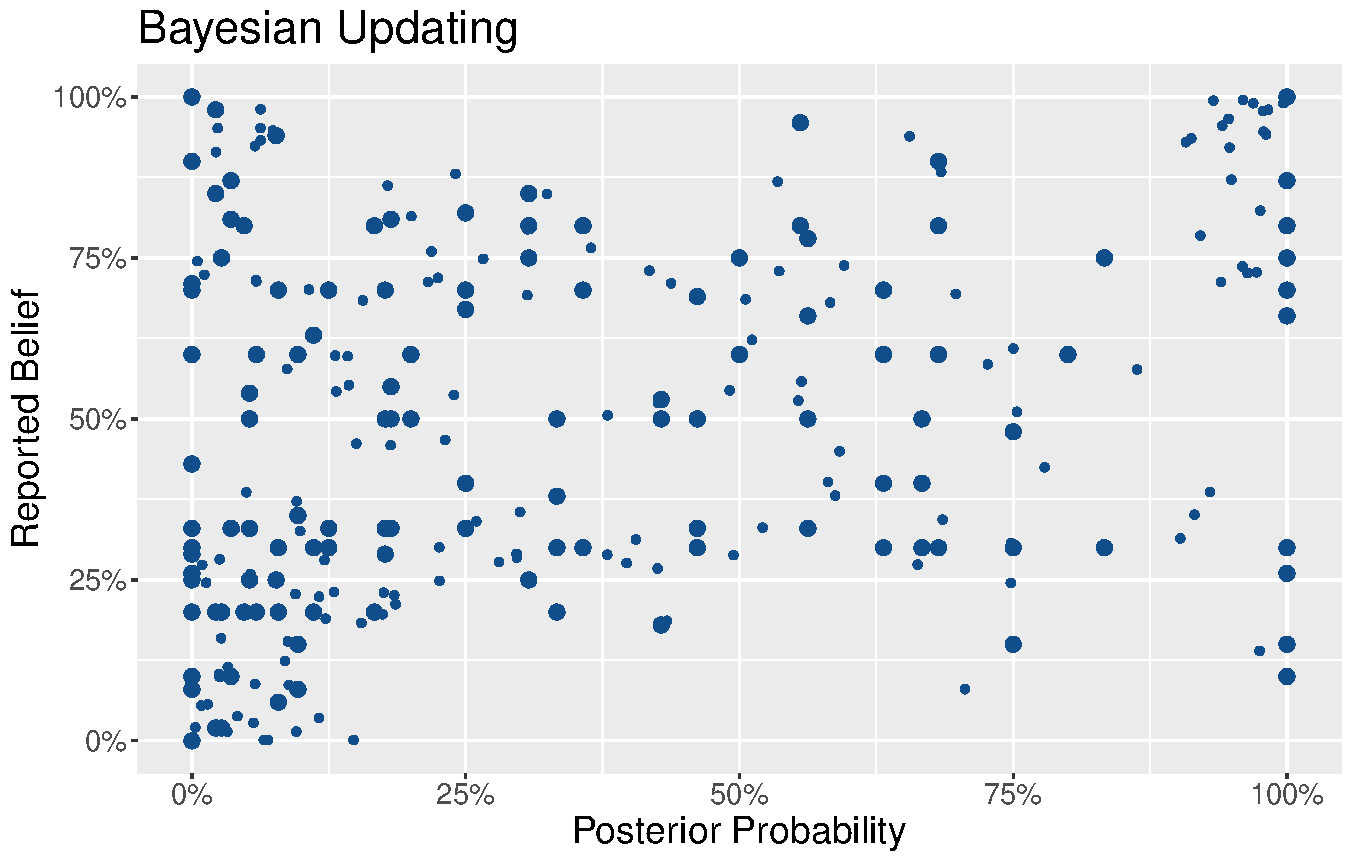
\includegraphics[scale=0.4]{Graphs/UPD_curve2.pdf}
\end{figure}
\end{frame}

\begin{frame}
\frametitle{Belief Updating: Correlation}
\footnotesize
\begin{table}[htbp]\centering
\def\sym#1{\ifmmode^{#1}\else\(^{#1}\)\fi}
\caption{Belief Elicitation: Belief vs Posterior}
\begin{tabular}{l*{3}{c}}
\hline\hline
                &\multicolumn{1}{c}{(1)}&\multicolumn{1}{c}{(2)}&\multicolumn{1}{c}{(3)}\\
                &\multicolumn{1}{c}{All}&\multicolumn{1}{c}{Not\_honest}&\multicolumn{1}{c}{Good quiz}\\
\hline
Posterior prob. &     .669\sym{***}&     .711\sym{***}&     .523\sym{***}\\
                &   (29.0)         &   (29.1)         &   (15.7)         \\
Constant        &     .151\sym{***}&     .147\sym{***}&     .226\sym{***}\\
                &   (16.2)         &   (14.1)         &   (17.8)         \\
\hline
Observations    &      780         &      636         &      520         \\
Adjusted \(R^{2}\)&     0.57         &     0.61         &     0.39         \\
\hline\hline
\multicolumn{4}{l}{\footnotesize \textit{t} statistics in parentheses}\\
\multicolumn{4}{l}{\footnotesize \sym{*} \(p<0.10\), \sym{**} \(p<0.05\), \sym{***} \(p<0.01\)}\\
\end{tabular}
\end{table}


\end{frame}

\begin{frame}
\frametitle{What Affects Beliefs?}
\footnotesize
\begin{table}[htbp]\centering
\def\sym#1{\ifmmode^{#1}\else\(^{#1}\)\fi}
\caption{Belief Elicitation: Discrepancy}
\begin{tabular}{l*{6}{c}}
\hline\hline
                &\multicolumn{1}{c}{(1)}&\multicolumn{1}{c}{(2)}&\multicolumn{1}{c}{(3)}&\multicolumn{1}{c}{(4)}&\multicolumn{1}{c}{(5)}&\multicolumn{1}{c}{(6)}\\
                &\multicolumn{1}{c}{}&\multicolumn{1}{c}{}&\multicolumn{1}{c}{}&\multicolumn{1}{c}{}&\multicolumn{1}{c}{}&\multicolumn{1}{c}{}\\
\hline
FN rate         &     .016         &     .016         &    -.014         &    -.014         &   -.0562         &   -.0554         \\
                &    (0.1)         &    (0.1)         &    (0.1)         &    (0.1)         &    (0.1)         &    (0.1)         \\
FP rate         &     .919\sym{***}&     .919\sym{***}&     1.07\sym{***}&     1.07\sym{***}&     1.05\sym{***}&     1.05\sym{***}\\
                &    (0.1)         &    (0.1)         &    (0.1)         &    (0.1)         &    (0.1)         &    (0.1)         \\
Good quiz       &                  &                  &    .0469         &    .0673         &                  &                  \\
                &                  &                  &    (0.0)         &    (0.0)         &                  &                  \\
Good quiz $\times$ FN rate&                  &                  &    .0463         &    .0464         &                  &                  \\
                &                  &                  &    (0.1)         &    (0.1)         &                  &                  \\
Good quiz $\times$ FP rate&                  &                  &    -.286\sym{*}  &    -.284\sym{*}  &                  &                  \\
                &                  &                  &    (0.2)         &    (0.2)         &                  &                  \\
Stat. class     &                  &                  &                  &                  &  -.00193         &   -.0127         \\
                &                  &                  &                  &                  &    (0.0)         &    (0.0)         \\
Stat. class $\times$ FN rate&                  &                  &                  &                  &     .127         &     .126         \\
                &                  &                  &                  &                  &    (0.1)         &    (0.1)         \\
Stat. class $\times$ FP rate&                  &                  &                  &                  &    -.229         &    -.226         \\
                &                  &                  &                  &                  &    (0.2)         &    (0.2)         \\
Constant        &    -.076\sym{***}&   -.0656\sym{***}&    -.101\sym{***}&    -.102\sym{***}&   -.0751\sym{***}&   -.0563         \\
                &    (0.0)         &    (0.0)         &    (0.0)         &    (0.0)         &    (0.0)         &    (0.0)         \\
Prior prob dummies &       No         &      Yes         &       No         &      Yes         &       No         &      Yes         \\
\hline
Observations    &      630         &      630         &      630         &      630         &      630         &      630         \\
Adjusted \(R^{2}\)&     0.17         &     0.17         &     0.17         &     0.17         &     0.17         &     0.17         \\
\hline\hline
\multicolumn{7}{l}{\footnotesize Standard errors in parentheses}\\
\multicolumn{7}{l}{\footnotesize \sym{*} \(p<0.10\), \sym{**} \(p<0.05\), \sym{***} \(p<0.01\)}\\
\end{tabular}
\end{table}

\end{frame}

\begin{frame}
\frametitle{Belief Updating: Decomposition}
\begin{itemize}
\item Posterior probability $\mu=P(B|S=x)$ that the ball is black conditional on a hint $S=x$ can be written as:
$$\ln \left({\mu \over 1-\mu} \right)=\lambda_0+S_B+S_W$$
\item With $\lambda_0\equiv \ln(p/(1-p))$ representing (transformed) prior beliefs
\item And $S_B$, $S_W$ describing the effect of new evidence:
$$S_B\equiv I(S=B)\ln(P(s=B|B)/P(s=B|W))$$
$$S_W\equiv I(S=W)\ln((1-P(s=B|B))/(1-P(s=B|W))$$
\end{itemize}
\end{frame}


\begin{frame}
\frametitle{Belief Updating: Decomposition}
\footnotesize
\begin{table}[htbp]\centering
\def\sym#1{\ifmmode^{#1}\else\(^{#1}\)\fi}
\caption{Belief Elicitation: Decomposition}
\begin{tabular}{l*{3}{c}}
\hline\hline
                &\multicolumn{1}{c}{(1)}&\multicolumn{1}{c}{(2)}&\multicolumn{1}{c}{(3)}\\
                &\multicolumn{1}{c}{OLS}&\multicolumn{1}{c}{FE}&\multicolumn{1}{c}{Smart, FE}\\
\hline
lt\_prior        &     .178         &     .205\sym{**} &     .231\sym{**} \\
                &    (1.4)         &    (2.5)         &    (2.2)         \\
signalB         &   -.0835         &     .735\sym{**} &     .988\sym{**} \\
                &   (-0.2)         &    (2.5)         &    (2.5)         \\
signalW         &     .818\sym{***}&        0         &        0         \\
                &    (2.8)         &      (.)         &      (.)         \\
Constant        &     .332         &    -.471\sym{**} &    -.577\sym{**} \\
                &    (0.9)         &   (-2.7)         &   (-2.6)         \\
\hline
Observations    &       68         &       68         &       52         \\
Adjusted \(R^{2}\)&     0.16         &     0.20         &     0.25         \\
\hline\hline
\multicolumn{4}{l}{\footnotesize \textit{t} statistics in parentheses}\\
\multicolumn{4}{l}{\footnotesize \sym{*} \(p<0.10\), \sym{**} \(p<0.05\), \sym{***} \(p<0.01\)}\\
\end{tabular}
\end{table}

\end{frame}





\end{document}
